
\documentclass[a4paper,12pt,twoside]{article}
\usepackage[a4paper,top=20mm,bottom=20mm,inner=38mm,outer=19mm]{geometry}
\usepackage{graphicx}
\usepackage{float}
\usepackage{url}
\usepackage{listings}
\usepackage{subfigure}
\usepackage{cite}
\usepackage{amssymb}
\usepackage{parskip}
\usepackage{setspace}
\bibliographystyle{apalike} 
\begin{document}
\onehalfspacing

\begin{titlepage}
\clearpage
\vspace*{\fill}
\begin{center}
\begin{minipage}{.6\textwidth}
\centerline{\textbf{\huge Gathering Atmospheric Data}}
\centerline{\textbf{\large Using an Unmanned Air Vehicle}}
\centerline{\textit{Henry Miskin}}
\centerline{\textit{\today}}
\end{minipage}
\end{center}
\vspace{5cm}
\center
\textbf{Abstract}
\center
This report looks at three dimensional energy based path planning for unmanned air vehicles in a predetermined area, with particular consideration to quality of data produced.
\vfill

\clearpage
\end{titlepage}
\tableofcontents
\clearpage

\section{Introduction}
\label{sec:introduction}

The following section outline the process in which a minimum cost route through a sample space can be obtained that provides the best data collection quality

\section{Plane Properties}
\label{sec:plane_properties}

\begin{table}[width=\textwidth]
\centering
    \begin{tabular}{ccc}
    Name	& Wingspan	& height	\\
Plane 1	& 20m	& 5m	\\
Plane 3	& 40m	& 6m	\\

    \end{tabular}
\caption{Table of Plane Properties}
\label{tbl:table_of_plane_properties}
\end{table}

To considere th minimum cost of circumnavigating a particular route the specifications of a plane must be considered in table \ref{tbl:table_of_plane_properties} the properties of differnt planes is shown

\section{Energy Model}
\label{sec:energy_model}

\begin{equation}
\label{eq:energy_equation}
E=\alpha D + \beta H
\end{equation}

From these plane properties the following energy model has been definened in equation \ref{eq:energy_equation} where $\alpha$ and $\beta$ are coeficients that are determined by the plane. For the current plane shown in table \ref{tbl:table_of_plane_properties} $\alpha$ and $\beta$ take values of 10 and 6 respectively.

\section{Latin Hypercubes}
\label{sec:latin_hypercubes}

Latin hypercubes are sampling pland that provide the best space fillingness while limiting the total number of sampling points required. This is generally applied to testing of computer similations where the collection of each point is expensive. In this situation however the travel bertween the points the expensive component.

\begin{figure}[H]
	\centering
	
	\subfigure[10 Nodes]{
		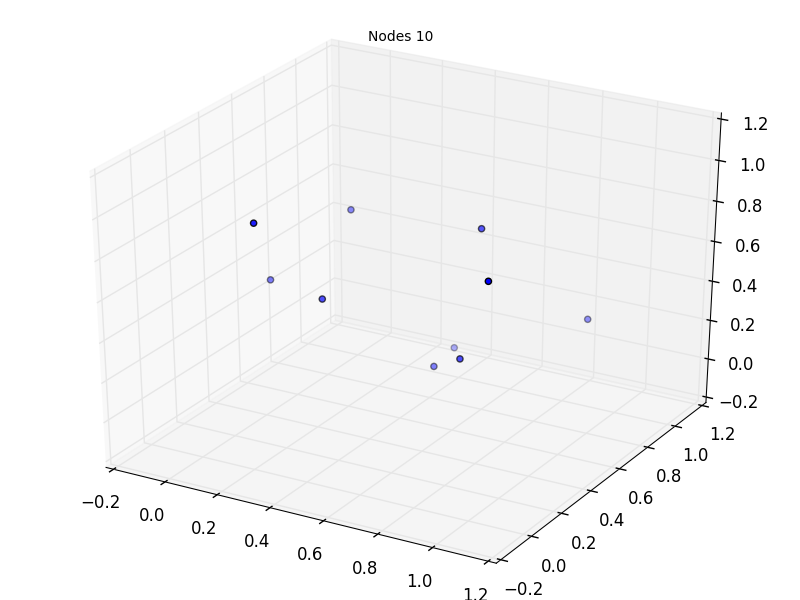
\includegraphics[width=0.4\textwidth]{figures/nodes_10.png} 
		\label{fig:10_nodes}
	}
	\subfigure[50 Nodes]{
		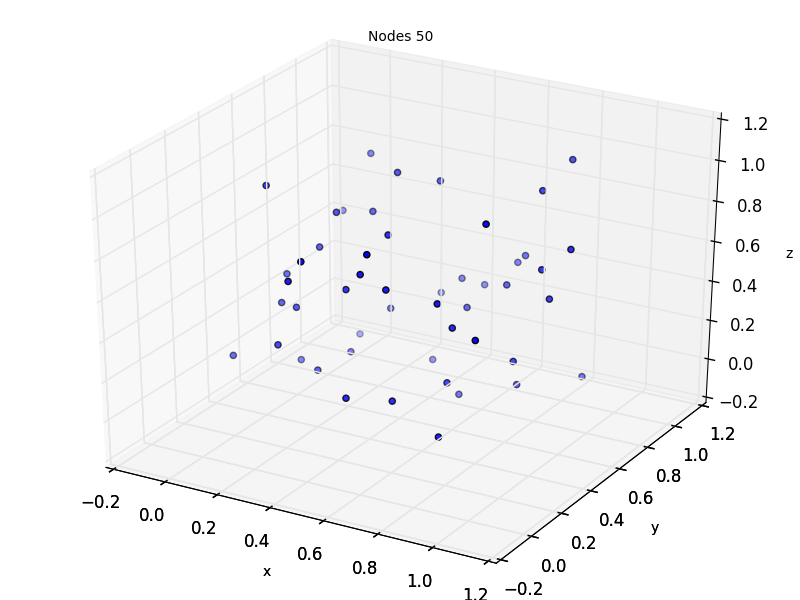
\includegraphics[width=0.4\textwidth]{figures/nodes_50.png} 
		\label{fig:50_nodes}
	}
	\subfigure[250 Nodes]{
		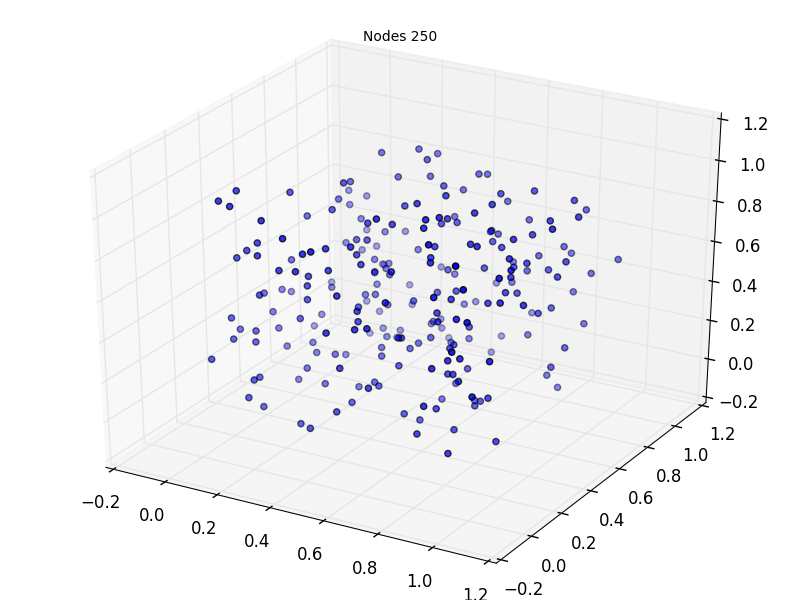
\includegraphics[width=0.4\textwidth]{figures/nodes_250.png} 
		\label{fig:250_nodes}
	}
	\subfigure[1250 Nodes]{
		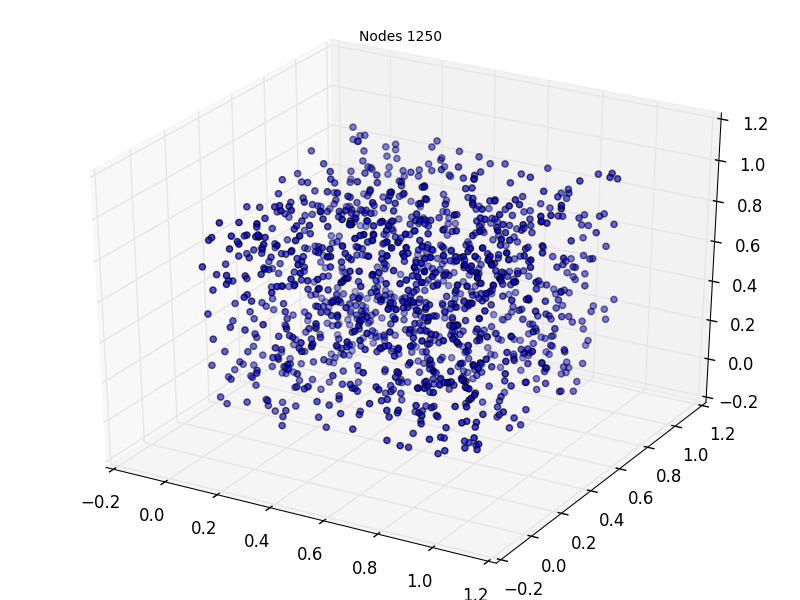
\includegraphics[width=0.4\textwidth]{figures/nodes_1250.png} 
		\label{fig:1250_nodes}
	}
	\caption{Latin Hypercubes with Varying Numbers of Nodes}
	\label{fig:latin_hypercubes_with_varying_numbers_of_nodes}
\end{figure}

Figure \ref{fig:latin_hypercubes_with_varying_numbers_of_nodes} shows a number of latin hypercubes with differnt numbers of nodes. All the Latin Hypercubes are within a unit cube. For collection of data in a required area these cubes can be stretched to fill the desired space. This does not provide an even spacing in each direction however means that eeach vertex of data collection is equally considered.

For this project the idea is to follow this logic to utilise Latin Hypercubes:

\begin{enumerate}
\item Specifiy area of interest to researcher
\item Estimate number of nodes able to be circumnavigated given the UAV total energy and the area of sample space
\item Fit Latin Hypercube of given nodes to sample area
\item Calcualte least energy route through the sample space
\item After first flight asses areas of encertainty to plan route through for next flight

\end{enumerate}

\section{Path Planning}
\label{sec:path_planning}

Given a set of points within a sample space the next stage of the proceedings is to compute the least cost path through these points. This problem presents itself in the forn of the travelling salesman problem. The travelling salesman problem is the problem of finding the least cost path through a set of points. There is lots of work done on the elicidean travelling salesman problem and introducing heroustics to improe the time taken to compute. This is due to the problem being an NP hard problem (the computing time required increases exponentially with the number of points in the route)

\begin{figure}[H]
	\centering
	
	\subfigure[4 Nodes]{
		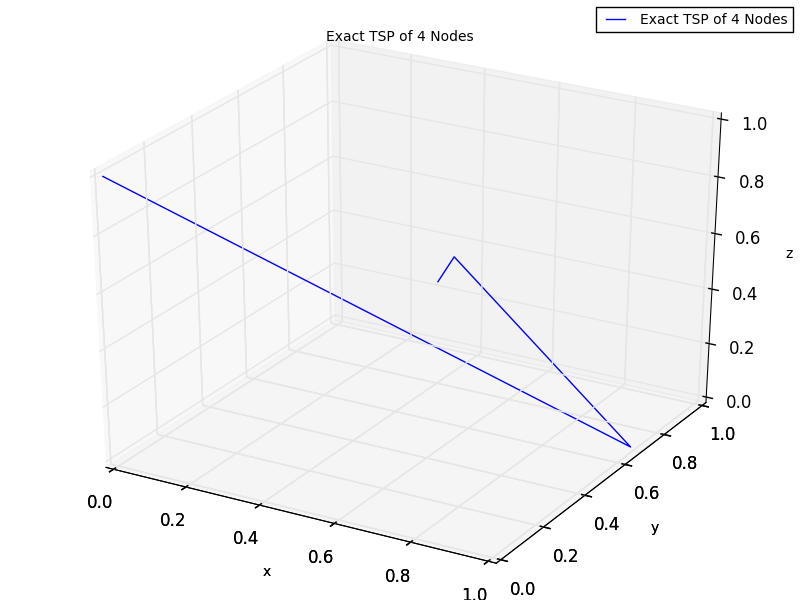
\includegraphics[width=0.4\textwidth]{figures/exact_tsp_of_4_nodes.png} 
		\label{fig:4_nodes}
	}
	\subfigure[6 Nodes]{
		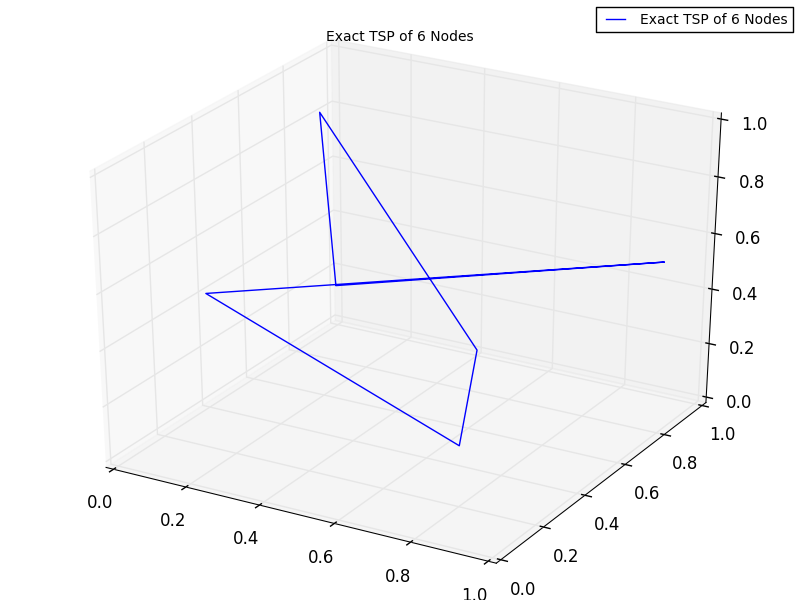
\includegraphics[width=0.4\textwidth]{figures/exact_tsp_of_6_nodes.png} 
		\label{fig:6_nodes}
	}
	\subfigure[8 Nodes]{
		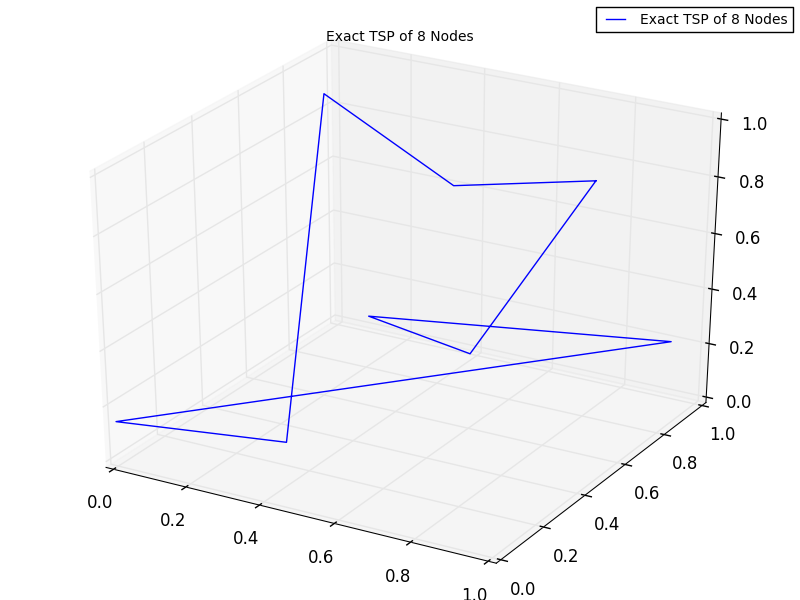
\includegraphics[width=0.4\textwidth]{figures/exact_tsp_of_8_nodes.png} 
		\label{fig:8_nodes}
	}
	\subfigure[10 Nodes]{
		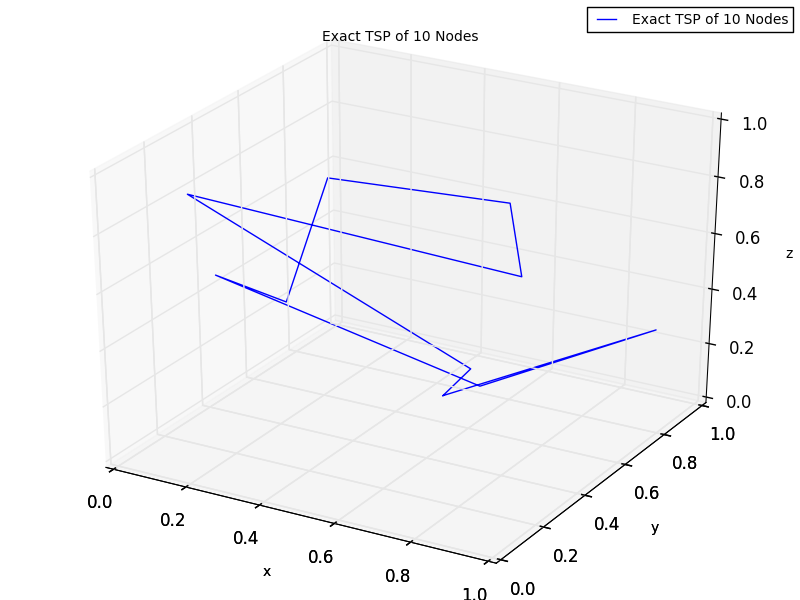
\includegraphics[width=0.4\textwidth]{figures/exact_tsp_of_10_nodes.png} 
		\label{fig:10_nodes}
	}
	\caption{Exact routes calculated by travelling salesman}
	\label{fig:exact_routes_calculated_by_travelling_salesman}
\end{figure}

Figure \ref{fig:exact_routes_calculated_by_travelling_salesman} shows the optimal routes for differnt numbers of nodes

\begin{table}[width=\textwidth]
\centering
    \begin{tabular}{lllll}
    Number of points	& 4	& 6	& 8	& 10	\\
Number of possible routes	& 24	& 720	& 40320	& 3628800	\\
Computation time (ms)	& 0.0	& 5.0	& 634.0	& 33670.0	\\
Best route cost (J)	& 110.38	& 106.71	& 106.72	& 108.76	\\

    \end{tabular}
\caption{Comparison of route calculation}
\label{tbl:comparison_of_route_calculation}
\end{table}

\begin{figure}[H]
\centering
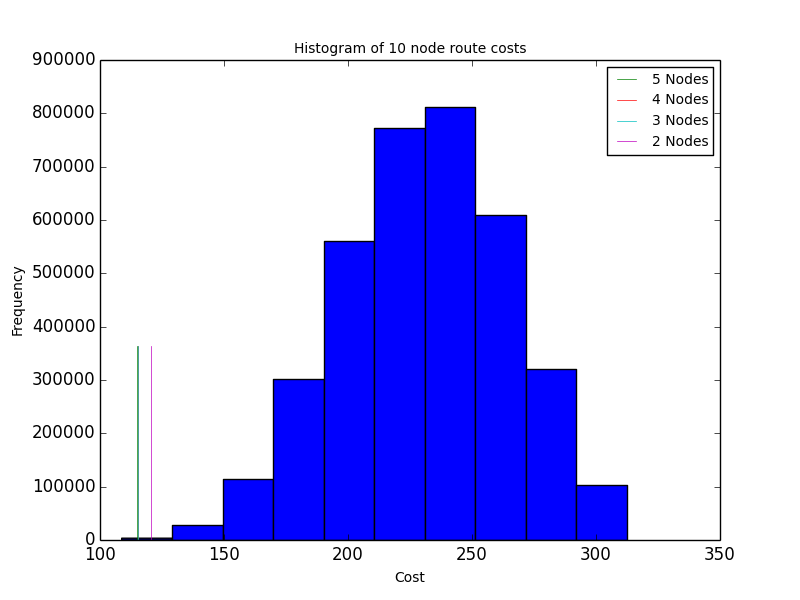
\includegraphics[width=0.4\textwidth]{figures/histogram_of_10_node_route_costs.png} 
\caption{Histogram of 10 node route costs}
\label{fig:histogram_of_10_node_route_costs}
\end{figure}

Figure \ref{fig:histogram_of_10_node_route_costs} shows a histogram of differnt route costs for a 10 node latin hypercube

\end{document}
